% =========================================================
% CONFIGURACION DEL DOCUMENTO
% =========================================================
\providecommand{\main}{..}
\documentclass[\main/Main.tex]{subfiles}

% =========================================================
% CONTENIDO
% =========================================================
\begin{document}
	\chapter{Lógica del script de ejecución}
	\label{cha:a01_script}
		A continuación se muestra de forma general el funcionamiento del script de ejecución para los experimentos:
		\begin{figure}[H]
            \centering
            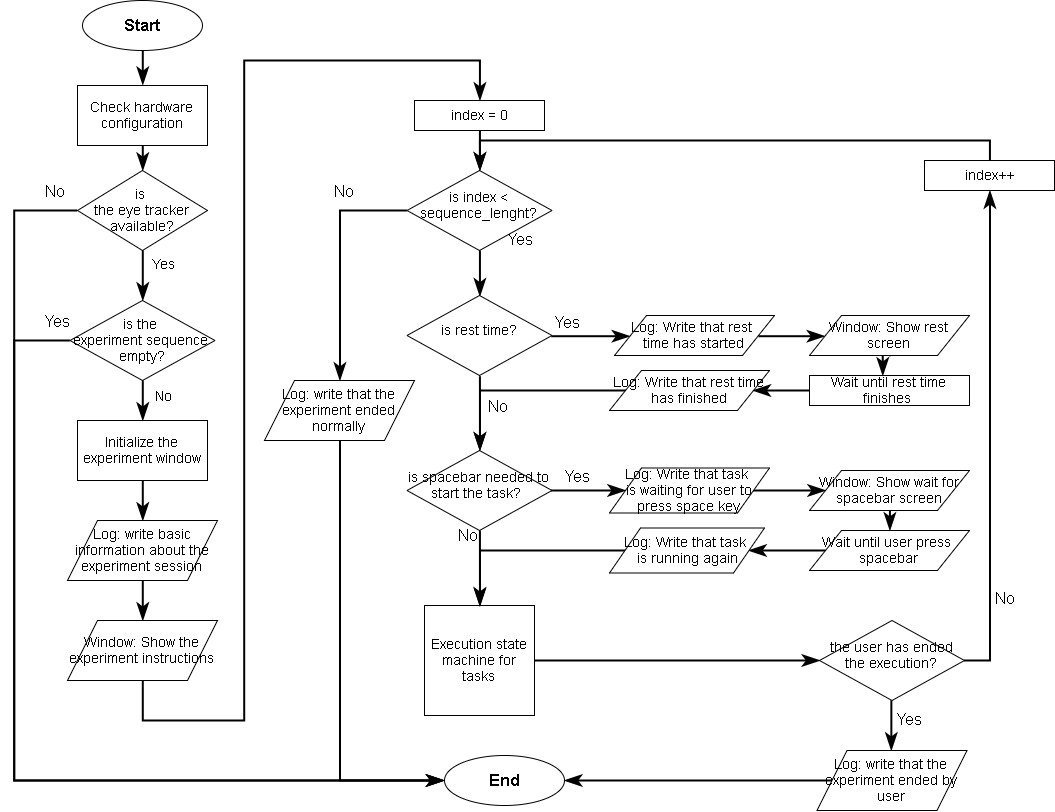
\includegraphics[width=\textwidth]{extra_01_script_base}
            \caption{Funcionamiento general del \textit{script} de ejecución.}
            \label{fig:a01_script}
        \end{figure} 

	\chapter{Configuración del entorno de programación}
	\label{cha:a02_install}
		Para el correcto funcionamiendo de \textit{psychoPy} y por tanto, de esta aplicación, es necesaria la instalación de una serie de herramientas de software. Para un sistema con Windows de 64-bit es necesario instalar:
		\begin{enumerate}\setlength\itemsep{-0.5em}		
			\item Librería para descodificación de video y audio AVbin10 en sus versiones de 32-bit y 64-bit. Descargar \href{http://avbin.github.io/AVbin/Download.html}{Aquí}. 
			\item Reproductor multimedia VLC en su versión de 32-bit. Descargar \href{https://www.videolan.org/vlc/download-windows.es.html}{Aquí}. 
			\item Compilador de Microsoft Visual C++ para Python 2.7. Descargar \href{https://www.microsoft.com/en-us/download/details.aspx?id=44266}{Aquí}. 
			\item Se necesita instalar la distribución Anaconda para uso con Python 2.7 en su versión de 32-bit. \href{https://www.anaconda.com/download/#download}{Aquí}. 
			\item Sobre la instalación de Anaconda debe crearse el siguiente entorno de programación: 
			\singlespacing{
				\pythonExternal{condaEnv_psychoPy_1.84.2_no-builds_win.yml}
			}
			Al cual debe incluirse el módulo ''pyHook'' en su versión 1.5.1 (descargar \href{https://www.lfd.uci.edu/~gohlke/pythonlibs/#pyhook}{Aquí}). 
		\end{enumerate}
\end{document}